\begin{wrapfigure}{r}{0.5\textwidth}
    \centering
    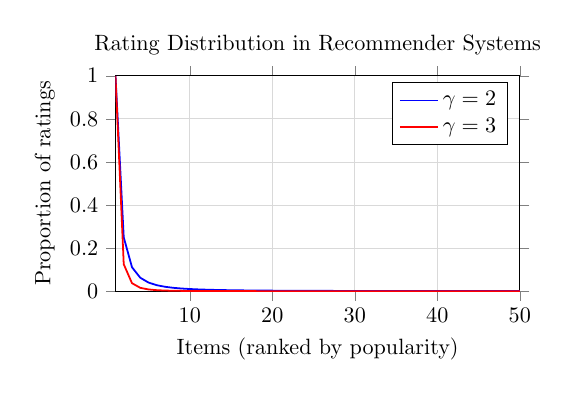
\begin{tikzpicture}[scale=0.8]
        \begin{axis}[
            xlabel={Items (ranked by popularity)},
            ylabel={Proportion of ratings},
            title={Rating Distribution in Recommender Systems},
            xmin=1, xmax=50,
            ymin=0, ymax=1,
            grid=major,
            grid style={gray!30},
            width=8cm,
            height=5cm,
            legend pos=north east,
            tick align=outside,
        ]
        
        % Power law with gamma = 2
        \addplot[
            blue,
            thick,
            domain=1:100,
            samples=100
        ] {x^(-2)};
        \addlegendentry{$\gamma = 2$}
        
        % Power law with gamma = 3
        \addplot[
            red,
            thick,
            domain=1:100,
            samples=100
        ] {x^(-3)};
        \addlegendentry{$\gamma = 3$}
        
        \end{axis}
    \end{tikzpicture}
    \caption{Power law distribution of ratings in recommender systems with $\gamma = 2$ and $\gamma = 3$.}
    \label{fig:power_law}
\end{wrapfigure}